\begin{enumerate}
  \item Definiční obor
  \item Derivace
  \item Nulové body
    \begin{enumerate}[label=(\alph*)]
      \item dosadit do derivace
      \item znaménko
    \end{enumerate}
  \item pouze v nul. bodech jsou extrémy
    \begin{itemize}
      \item může jich být více
      \item ostré lokální maximu, minimum
    \end{itemize}
\end{enumerate}
\subsubsection{Lokální extrémy - příklady}
\begin{align}
  f(x)=x^4-8x^2+16
\end{align}
\hrule
\begin{center}
  Podmínky: $D(f)=\mathbb{R}$
\end{center}
\begin{align*}
  f'(x)=4x^3-16=4x*(x^2-4)=0 \\
  \begin{alignedat}{2}
    \text{nulové body  }\,
    \Biggr|\,
    \begin{alignedat}{2}
      4x &=0 \quad x_1 \rightarrow &0 \\
      x^2-4 &=0 \quad x_2 \rightarrow &\pm2 \\
    \end{alignedat}
    \,\Biggr|
  \end{alignedat}
\end{align*}
\begin{center}
  \begin{tabular}{l}
    ostré lokální maximum v $x=0$\\
    ostré lokální minimum v $x=-2$\\
    ostré lokální minimum v $x=2$
  \end{tabular}
\end{center}
\begin{center}
  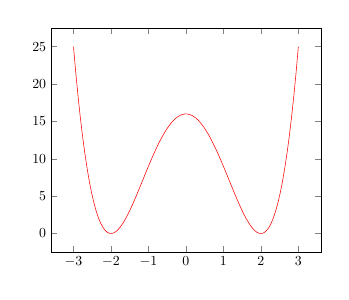
\begin{tikzpicture}[scale=0.5]
    \begin{axis}
      \addplot[color=red,domain=-3:3,samples=100]{x^4-8*x^2+16};
    \end{axis}
  \end{tikzpicture}
\end{center}

